\documentclass[11pt]{article}
\usepackage[utf8]{inputenc}
\usepackage[T1]{fontenc}
\usepackage[english]{babel}
\usepackage{amsmath, amssymb, amsthm}
\usepackage{graphicx}
\usepackage{geometry}
\usepackage{array}
\usepackage{booktabs}
\usepackage{float}
\usepackage{setspace}
\geometry{a4paper, margin=1in}
\usepackage{hyperref}
\usepackage{tikz}
\usetikzlibrary{positioning}
\usepackage{tkz-graph}
\usetikzlibrary{arrows, calc}
\usepackage{booktabs}
\usepackage{multirow}
\usepackage{multicol}
\usepackage[super]{cite}

\usepackage{xcolor} % Pour les couleurs
%\usepackage[margin=0.5cm]{geometry} % Réduction des marges
\usepackage{pgfgantt}
\usepackage{adjustbox} 

\usepackage{amsmath,amssymb}
\usetikzlibrary{arrows.meta,positioning,calc}

\usepackage{dirtree}



% Nouvelle commande pour dessiner un réseau de neurones
% Argument : une liste de nombres, par exemple {4,5,5,5,3}
% Chaque nombre représente le nombre de neurones dans la couche correspondante
\newcommand{\drawNeuralNetwork}[4]{%
    \def\layers{#1}
    \def\nodesize{#2}
    \def\scalex{#3}
    \def\scaley{#4}

    % Style des neurones
    \tikzstyle{mynode}=[thick,draw=black,fill=white!20,circle,minimum size=\nodesize]

    \begin{tikzpicture}[x=\scalex,y=\scaley]
        \foreach \N [count=\lay,remember={\N as \Nprev (initially 0)}] in \layers {
            \foreach \i [evaluate={\y=\N/2-\i; \x=\lay; \prev=int(\lay-1);}] in {1,...,\N} {
                \node[mynode] (N\lay-\i) at (\x,\y) {};
                \ifnum\Nprev>0
                    \foreach \j in {1,...,\Nprev}{
                        \draw[thick] (N\prev-\j) -- (N\lay-\i);
                    }
                \fi
            }
        }
    \end{tikzpicture}
}



%%%%%%%%%%%%%%%%%%  stack exhange code pour arbre

\usepackage[edges]{forest}
\definecolor{folderbg}{RGB}{124,166,198}
\definecolor{folderborder}{RGB}{110,144,169}
\newlength\Size
\setlength\Size{4pt}
\tikzset{%
  folder/.pic={%
    \filldraw [draw=folderborder, top color=folderbg!50, bottom color=folderbg] (-1.05*\Size,0.2\Size+5pt) rectangle ++(.75*\Size,-0.2\Size-5pt);
    \filldraw [draw=folderborder, top color=folderbg!50, bottom color=folderbg] (-1.15*\Size,-\Size) rectangle (1.15*\Size,\Size);
  },
  file/.pic={%
    \filldraw [draw=folderborder, top color=folderbg!5, bottom color=folderbg!10] (-\Size,.4*\Size+5pt) coordinate (a) |- (\Size,-1.2*\Size) coordinate (b) -- ++(0,1.6*\Size) coordinate (c) -- ++(-5pt,5pt) coordinate (d) -- cycle (d) |- (c) ;
  },
}
\forestset{%
  declare autowrapped toks={pic me}{},
  pic dir tree/.style={%
    for tree={%
      folder,
      font=\ttfamily,
      grow'=0,
    },
    before typesetting nodes={%
      for tree={%
        edge label+/.option={pic me},
      },
    },
  },
  pic me set/.code n args=2{%
    \forestset{%
      #1/.style={%
        inner xsep=2\Size,
        pic me={pic {#2}},
      }
    }
  },
  pic me set={directory}{folder},
  pic me set={file}{file},
}

%%%%%%%%%%%%%%%%    

%%%%%%%%%%%%%%%%%   Il faut pas qu'on oublie la conclusion a chaque partie    %%%%%%%%%%%%%%%%%%%%

\begin{document}




%\thispagestyle{empty}

\begin{center}

    
\includegraphics[width=0.5\textwidth]{PageGarde/junia.png}\\[1cm]

    {\Large \textbf{Technical Report}}\\[1cm]


    % Ligne horizontale
    \rule{\textwidth}{0.5pt}\\[0.8cm]
    {\Huge \textbf{Accelerating Donor Material Discovery Using Machine Learning : A Deep Neural Network Approach}}\\[0.8cm]
    \rule{\textwidth}{0.5pt}\\[2cm]

    \textbf{Members :}\\
    \textsc{AMADOU SOUMANOU Omonlabakè Raliatou}\\
    \textsc{CHERIF Wissem}\\
    \textsc{CODO Loth-Marie Jg}\\
    \textsc{MEVAH MBELLE Marlene Tatiana}\\
    \textsc{RAOUMBE Axel}\\[3cm]

    \textbf{Supervised by :}\\
    \textsc{Kekeli N'KONOU}\\[1cm] % Nom de l'encadrant

    \vfill

    

    %\begin{minipage}{0.45\textwidth}
    %\begin{flushleft}
    %\textbf{Author:}\\
    %John Smith
    %\end{flushleft}
    %\end{minipage}
    %\hfill
    %\begin{minipage}{0.45\textwidth}
    %\begin{flushright}
    %\textbf{Supervisor:}\\
    %Dr.\ James Smith
    %\end{flushright}
    %\end{minipage}

    %\vfill
    {\large \textsc{Academic year : 2024 – 2025}}
    
\end{center}



\newpage

\tableofcontents 

\newpage

\section{Introduction}
\subsection{Contexte}
La découverte de nouveaux matériaux joue un rôle central dans l'accélération de l'innovation technologique, en particulier dans le domaine de l'efficacité énergétique. 
Alors que la demande mondiale de solutions énergétiques durables augmente, les cellules solaires organiques (OSC) apparaissent comme une alternative prometteuse aux cellules photovoltaïques traditionnelles. 
Ces dispositifs se distinguent par leurs nombreux avantages, notamment leur faible coût de fabrication, leur flexibilité mécanique, leur facilité de production à grande échelle et leur faible toxicité. Cependant, l'amélioration de l'efficacité de la conversion de puissance (PCE) reste un défi majeur.

La qualité des matériaux constituant la couche active des OSC, composée de matériaux donneurs (polymères et petites molécules) et d'accepteurs, est un facteur décisif de leur performance. La découverte et l'optimisation de matériaux donneurs performants nécessitent des cycles expérimentaux longs, coûteux et gourmands en ressources, ce qui entrave l'adoption généralisée de cette technologie.

Dans ce contexte, l'intégration de techniques d'apprentissage automatique, en particulier l'apprentissage profond, offre une solution innovante. Celles-ci peuvent modéliser des données complexes et temporelles, ce qui les rend particulièrement adaptées à la prédiction des propriétés des matériaux et à la génération de nouvelles structures moléculaires optimisées pour maximiser le PCE.

\subsection{Objectifs du projet}
L'objectif principale de ce projet est d'accélérer la découverte de nouveaux matériaux donneurs pour les OSC en utilisant des techniques d'apprentissage automatique. 
En particulier, nous visons à développer un modèle basé sur l'apprentissage profond capable de prédire efficacement le PCE des matériaux donneurs. 
En parallèle, nous utiliserons des algorithmes de génération moléculaire pour créer de nouvelles structures moléculaires optimisées pour les OSC.
En vu du développement de ce projet, nous écrivons un rapport technique dans le but de permettre à quiconque de prendre en main le modèle d'apprentissage développé et de l'utiliser pour prédire les propriétés des matériaux donneurs, en particulier le PCE.

\newpage

\section{Architecture du modèle}

Pour répondre à la problématique de la découverte de nouveaux matériaux donneurs pour les OSC, 
nous nous appuyons sur les travaux de \textbf{Jinyu Sun et al. \cite{Sun}} qui ont développé un modèle d'apprentissage profond pour la génération de molécules et du QuantumDeepField de \textbf{Masashi et al. \cite{Masashi}} capable de prédire les propriétés électroniques des molécules. 

\subsection{Modèle de prédiction de propriétés (PCE)}

Dans ce modèle, nous parlerons du \textbf{Quantum Deep Field} (QDF) pour prédire les propriétés des matériaux donneurs telles que le PCE.
L'architecture du modèle repose sur deux réseaux de neuronnes profonds majeures : le réseau de neurones de prédiction de propriétés et le réseau de neurones basés sur des contraintes physiques.
L'architecture du modèle est illustrée ci-dessous. \\


\begin{figure}[htbp]
    \centering
    \resizebox{\linewidth}{!}{
        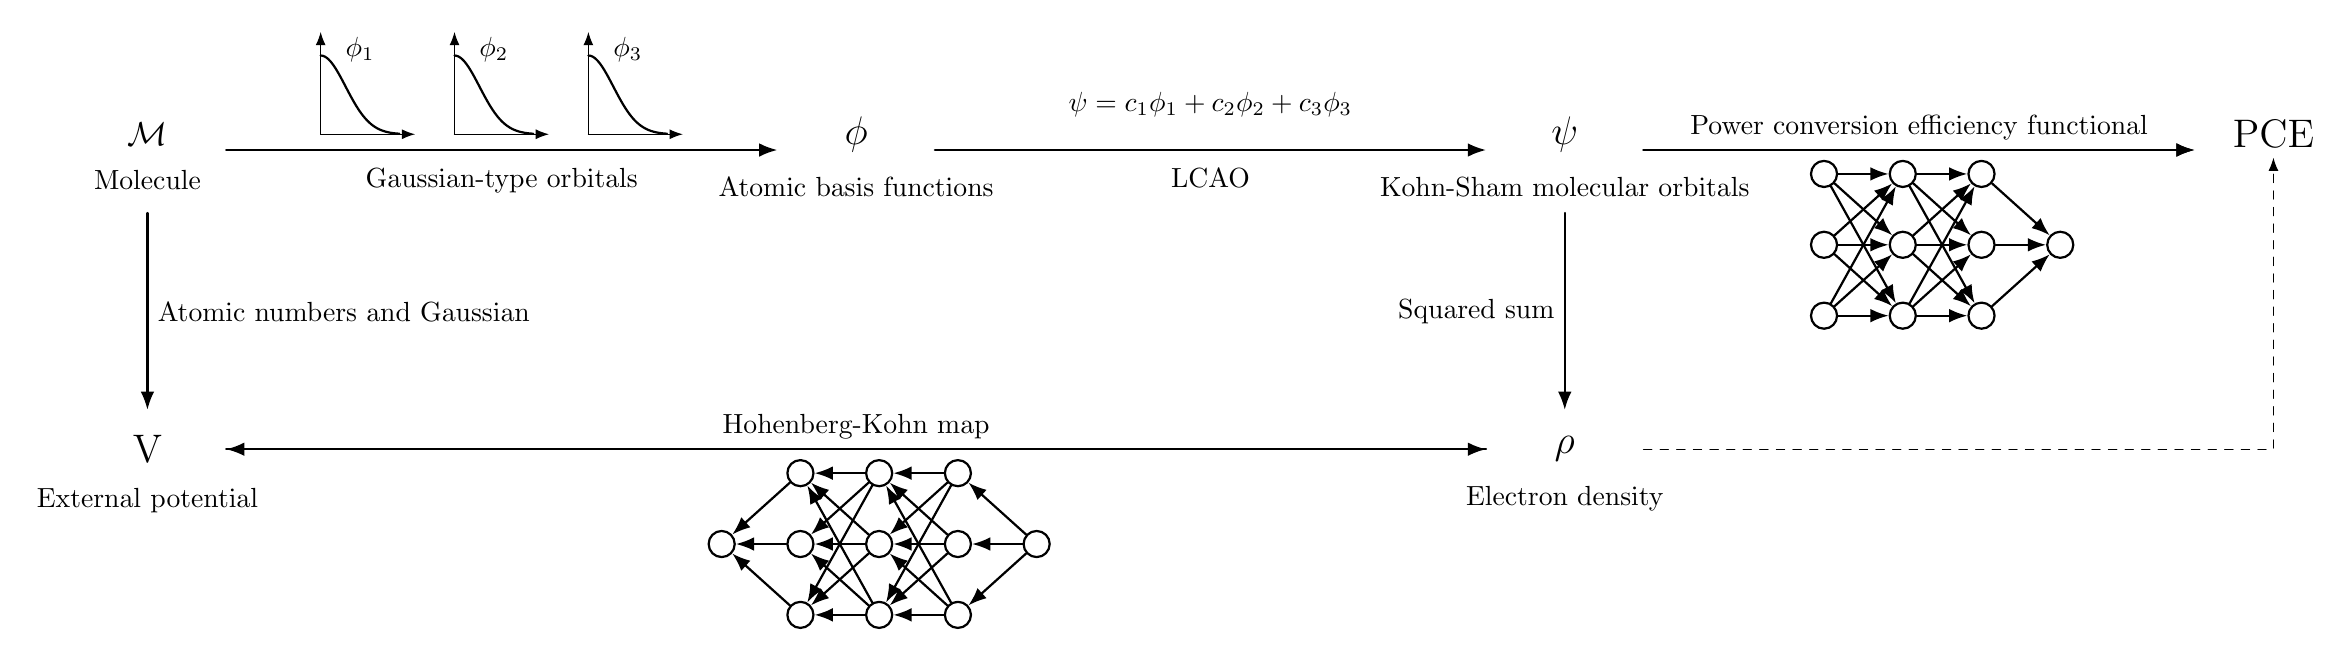
\begin{tikzpicture}[ >=Latex,  % Pour les pointes de flèche
            line cap=round, line join=round,  % Bords arrondis
            wavefn/.style={thick}    % Style pour tracer les fonctions
        ]
        
        % (1) Le « M » stylisé et l'étiquette "Molecule"
        \node[font=\large] (M) at (0,0) {$\mathcal{M}$};
        \node[below=2pt of M] {Molecule};
        
        % (2) Grande flèche horizontale (à droite du M)
        \draw[thick,->] (1,-0.2) -- ++(7,0)
            node[midway, below=3pt]{Gaussian-type orbitals};
        
        % (3) Tracer les trois "orbitales" gaussiennes
        % Première orbitale φ1
        \begin{scope}[xshift=2.2cm, yshift=0cm]
            \draw[->] (0,0) -- (0,1.3);
            \draw[->] (0,0) -- (1.2,0);
            \draw[domain=0:1.0, samples=40, wavefn]
            plot (\x,{1.0*exp(-5*(\x)^2)});
            \node[above] at (0.5,0.8) {$\phi_1$};
        \end{scope}
        
        % Deuxième orbitale φ2
        \begin{scope}[xshift=3.9cm, yshift=0cm]
            \draw[->] (0,0) -- (0,1.3);
            \draw[->] (0,0) -- (1.2,0);
            \draw[domain=0:1.0, samples=40, wavefn]
            plot (\x,{1.0*exp(-5*(\x)^2)});
            \node[above] at (0.5,0.8) {$\phi_2$};
        \end{scope}
        
        % Troisième orbitale φ3
        \begin{scope}[xshift=5.6cm, yshift=0cm]
            \draw[->] (0,0) -- (0,1.3);
            \draw[->] (0,0) -- (1.2,0);
            \draw[domain=0:1.0, samples=40, wavefn]
            plot (\x,{1.0*exp(-5*(\x)^2)});
            \node[above] at (0.5,0.8) {$\phi_3$};
        \end{scope}
        
        % Étiquette "Atomic basis functions"
        \node[font=\Large] (phi) at (9,0) {$\mathcal{\phi}$};
        \node[below=2pt of phi] {Atomic basis functions};
        
        \draw[thick,->] (10,-0.2) -- ++(7,0)
            node[midway, below=3pt]{LCAO};
        
        % L'équation LCAO
        \node[above] at (13.5,0.1) {$\psi = c_{1}\phi_{1} + c_{2}\phi_{2} + c_{3}\phi_{3}$};
        
        \node[font=\Large] (psi) at (18,0) {$\mathcal{\psi}$};
        \node[below=2pt of psi] {Kohn-Sham molecular orbitals};
        
        \draw[->, thick] (18,-1) -- (18, -3.5) node[midway, left] {Squared sum};
        
        \node[font=\Large] (rho) at (18,-4) {$\mathcal{\rho}$};
        \node[below=2pt of rho] {Electron density};
        
        \draw[->, thick] (17,-4) -- (1, -4) node[midway, above] {Hohenberg-Kohn map};
        
        \draw[<-, thick] (17,-4) -- (1, -4) node[midway, below] {\drawNeuralNetwork{1,3,3,3,1}{1pt}{1cm}{0.9cm}};

        % External potential
        \node[font=\Large] (V) at (0,-4) {V};
        \node[below=2pt of V] {External potential};
        
        \draw[->, thick] (0,-1) -- (0, -3.5) node[midway, right] {Atomic numbers and Gaussian};
        
        \draw[->, thick] (19, -0.2) -- ++ (7, 0) node[midway, above] {Power conversion efficiency functional};

        \draw[->, thick] (19, -0.2) -- ++ (7, 0) node[midway, below] {\drawNeuralNetwork{3,3,3,1}{1pt}{1cm}{0.9cm}};
        
        \node[font=\Large] (PCE) at (27,0) {PCE};
        
        \draw[dashed, ->] ($(rho)+(1,0)$) -| (PCE);
        
        \end{tikzpicture}
    }
    \caption{Quantum Deep Field (QDF) pour la prédiction de PCE}
    \label{fig:architecture}
\end{figure}


% \paragraph{Étape 1 \: Représentation de la molécule } 
\subsubsection{Représentation de la molécule}
La molécule d’intérêt, notée $\mathcal{M}$, est d’abord représentée sous forme de coordonnées atomiques et de numéros atomiques. Cette représentation sert de point de départ pour la génération des fonctions de base atomiques.

% \paragraph{Étape 2 \: Construction des orbitales atomiques de type gaussien} 
\subsubsection{Construction des orbitales atomiques de type gaussien}
À partir de la structure moléculaire, des orbitales atomiques de type gaussien ($\phi_1$, $\phi_2$, $\phi_3$, ...) sont générées. Ces fonctions de base servent à décrire la distribution électronique autour de chaque atome.

\subsubsection{Combinaison linéaire des orbitales atomiques (LCAO)}
Les orbitales atomiques sont combinées linéairement pour former les orbitales moléculaires de Kohn-Sham ($\psi$), selon la méthode LCAO ($\psi = c_1\phi_1 + c_2\phi_2 + c_3\phi_3$). Cette étape permet de modéliser la structure électronique de la molécule.

\subsubsection{Densité électronique et HK\_map}
La densité électronique ($\rho$) est obtenue en sommant les carrés des orbitales moléculaires. Cependant, minimiser uniquement la fonction de perte $\mathcal{L}_{PCE}$ ne garantit pas que le modèle appris soit physiquement significatif. 

En effet, en raison de la forte non-linéarité du réseau de neurones profond (DNN), il est possible d'obtenir un PCE correcte même si les orbitales de Kohn-Sham $\psi$ ne sont pas valides. Cela signifie que le modèle ne garantit pas que les orbitales $\psi(\mathbf{r})$ produisent la bonne densité électronique $\rho(\mathbf{r}) = \sum_{n=1}^N |\psi_n(\mathbf{r})|^2$.

Pour remédier à ce problème, une contrainte supplémentaire est imposée sur $\psi(\mathbf{r})$ basée sur le théorème de Hohenberg-Kohn, qui assure que le potentiel externe $V(\mathbf{r})$ est une fonction unique de la densité électronique.

\subsubsection{PCE}
Le PCE est calculé à partir des orbitales moléculaires. Il est exprimé par un DNN, ce qui permet d'évaluer l'efficacité de conversion d'énergie de la molécule. \\

En somme, on a 2 prédictions princiaples effetuées par le modèle :
\begin{itemize}
    \item \textbf{Prédiction du potentiel $V(\mathbf{r})$} : La première, qui est une prédiction sur le potentiel,sert de contraintes physiques pour ajuster le modèle de prédiction de PCE.
    \item \textbf{Prédiction du PCE} : La deuxième prédiction est le PCE de la molécule.
\end{itemize}

\subsection{Modèle de genération de molécules}
Ce modèle repose sur une approche par modélisation générative utilisant
un Auto-Encodeur Variationnel (VAE), combinée à une préparation des
données chimiques. L'objectif est de créer un système capable de représenter
fidèlement les structures moléculaires dans un espace latent continu, puis d'utiliser
ces représentations pour générer de nouvelles structures prometteuses en termes
d'efficacité photovoltaïque

Le choix du VAE s'explique par sa capacité à encoder des données complexes dans
un espace latent structuré, tout en permettant la génération d'exemples nouveaux
par simple échantillonnage. Dans notre cas, cela permet de transformer des chaînes
SMILES en vecteurs continus, puis de régénérer des chaînes moléculaires viables à
partir de ces vecteurs. Le VAE est particulièrement utile pour éviter les erreurs
syntaxiques communes lors de la génération de nouvelles molécules.

Le modèle VAE utilisé dans ce projet se compose de trois parties principales :

\begin{itemize}
    \item \textbf{Encodeur} : transforme les SMILES vectorisés en une distribution latente gaussienne.
    \item \textbf{Espace latent} : échantillonnage dans cet espace pour produire des représentations moléculaires nouvelles.
    \item \textbf{Décodeur} : reconstruit des SMILES valides à partir des vecteurs latents.
\end{itemize}


\begin{figure}[H]
    \centering
    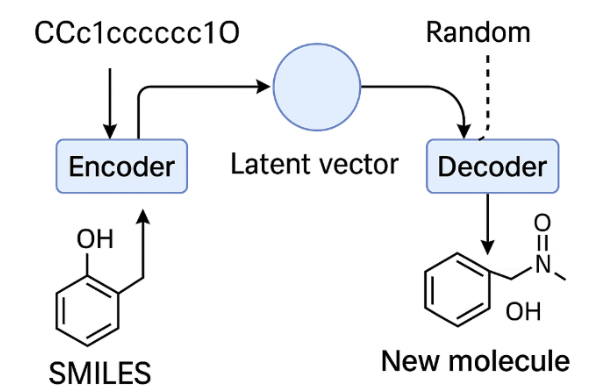
\includegraphics[width=0.4\textwidth]{Architecture/vae.png}
    \caption{Architecure VAE}
\end{figure}

Cette architecture permet non seulement de reproduire fidèlement les molécules du
dataset, mais aussi de générer des candidats inédits pour les OPV. \\

Chaque molécule passe par plusieurs étapes :

\begin{itemize}
    \item \textbf{Nettoyage des données} : vérification de l'intégrité des SMILES, suppression des anomalies et standardisation.
    \item \textbf{Vectorisation} : conversion caractère par caractère ou via des embeddings, pour produire des vecteurs traitables par les modèles.
    \item \textbf{Normalisation} : application de padding et de mise à l'échelle, pour assurer une homogénéité des entrées.
\end{itemize}

Ces transformations permettent au réseau d'extraire les caractéristiques pertinentes des molécules tout en préservant leur validité chimique.

\subsection{Architecure globale du modèle}

L'architecture globale du modèle combine les deux parties précédentes : le
modèle de prédiction de propriétés et le modèle de génération de molécules.

\begin{figure}[H]
    \centering
    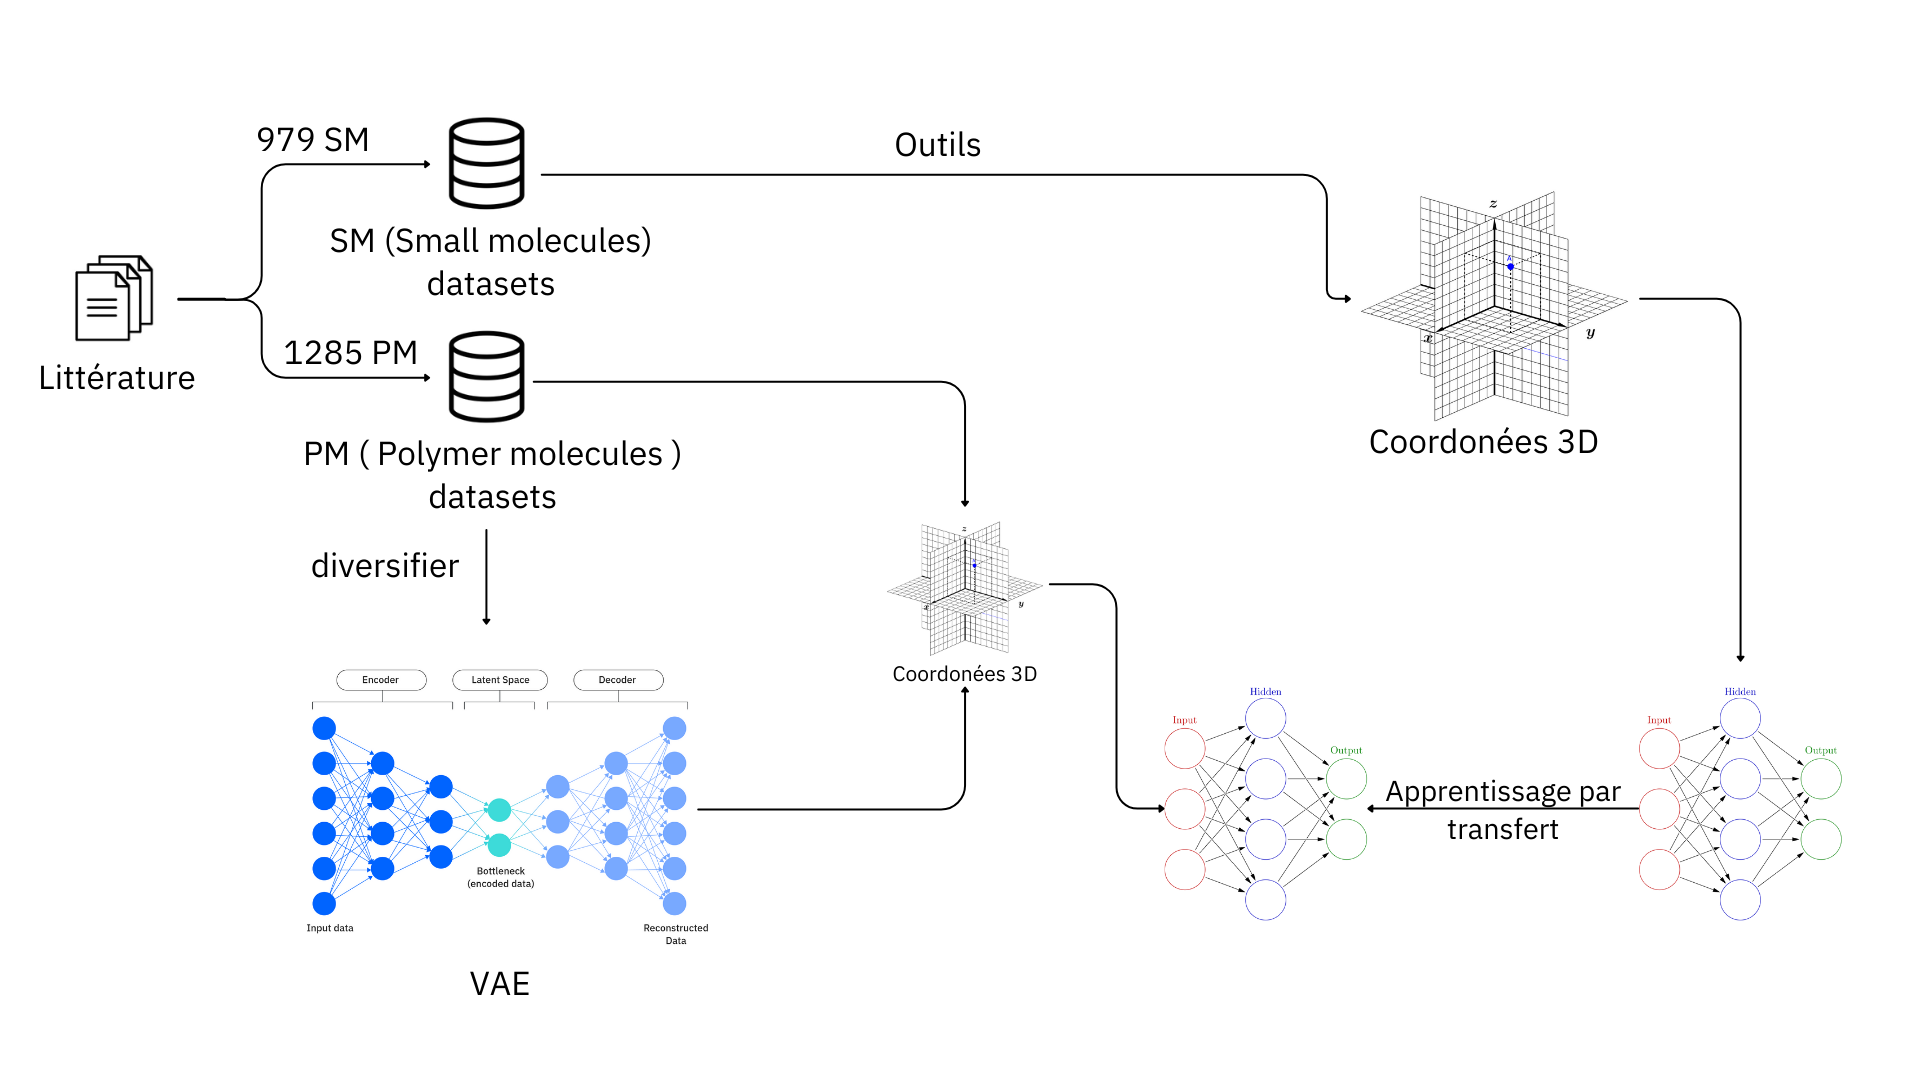
\includegraphics[width=0.8\textwidth]{Architecture/global.png}
    \caption{Architecure globale du modèle}
\end{figure}

On peut voir sur le modèle qu'il y a une série d'étape pour notre achitecture :
\begin{itemize}
    \item \textbf{Tranformations des molécules en 3D} : La première chose à faire est de transformer les molécules en coordonnées pour l'entrainement du modèle.
    \item \textbf{Entrainement du modèle QDF-SM} : Entrainer dans un premier le modèle sur les molécules SM tranformées.
    \item \textbf{Transfert Learning du modèle QDF-PM} : Faire de l'apprentissage par transfert sur les molécules PM tranformées.
    \item \textbf{Génération de molécules} : Génération de nouvelles molécules qui sont à tester sur les modèles entrainés (pour la prédiction).
\end{itemize}

En résumé, l’architecture proposée combine un modèle génératif basé sur un Auto-Encodeur Variationnel (VAE) pour la création de nouvelles structures moléculaires et un modèle de prédiction de propriétés (Quantum Deep Field) pour évaluer leur efficacité photovoltaïque. 
Cette approche intégrée permet non seulement d’explorer efficacement l’espace chimique à la recherche de nouveaux matériaux donneurs, mais aussi de prédire les propriétés de matériaux tels que le PCE.

\newpage

\section{Datasets}

\subsection{Overview sur les Datasets} 

Les datasets utilisés dans ce projet sont issus du dépôt GitHub de Jinyu Sun et al. \cite{Sun} sur le DeepDonor.
Dans ce dépôt on trouve deux types de datasets : SM (Small Molecules) et PM (Polymer Molecules). Pour pouvoir évalué le modèle plus tard il nous fallait les mêmes données que celles utilisées par Jinyu Sun et al. \cite{Sun}.

Le datset SM est constitué de \textbf{979 SM} tandis que le datasets PM est constitué de \textbf{1285 PM} et comportent des molécules qui proviennent de la littérature.
Ils sont sont au format \textbf{csv} et dans chacun d'eux on retrouve les molécules encodés en \textbf{SMILES} et leurs \textbf{PCE} respectifs.

\begin{figure}[htbp]
    \centering
    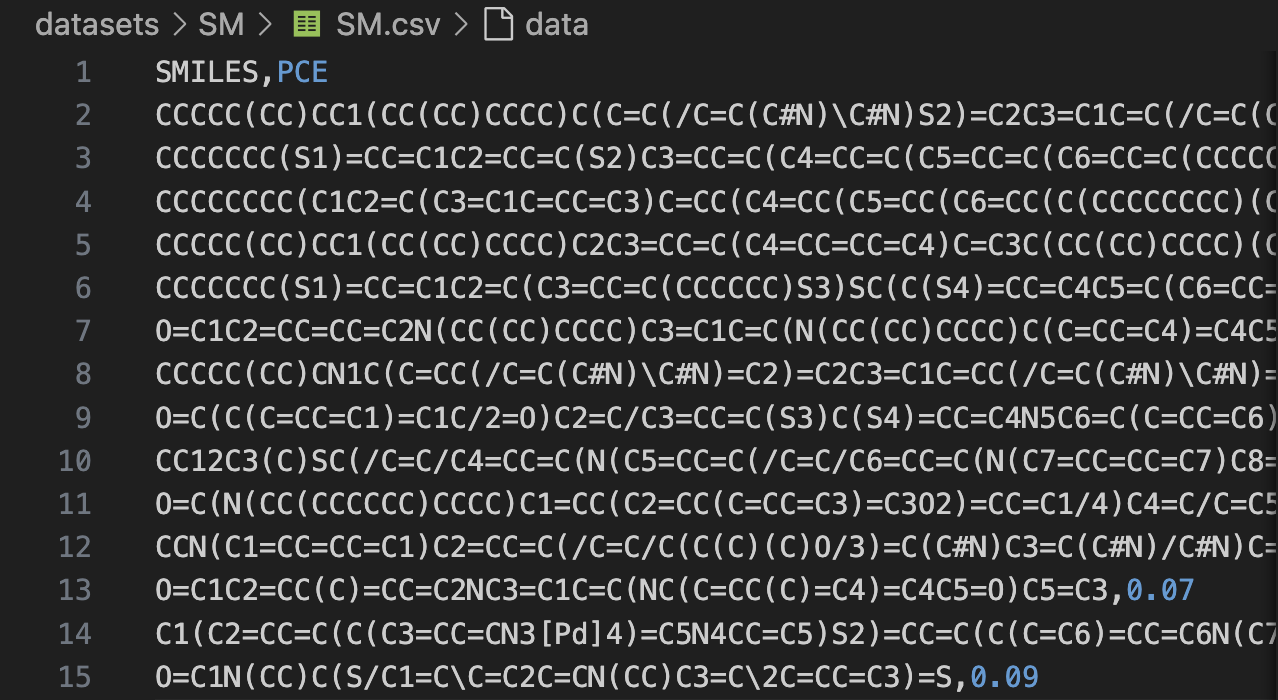
\includegraphics[width=0.6\textwidth]{Datasets/data.png}
    \caption{SMILES et PCE}
\end{figure}

Comme on peut le voir sur la figure ci-dessus, chaque ligne du fichier csv correspond à une molécule encodé en SMILES associées à leurs PCE respectif.

Un point important à noter est le fait qu'il y a une différence entre les PM et les SM. Cette différence réside au niveau de la masse moléculaires.
Ainsi, ce point est intéressant à prendre en compte pour éviter toute confusion pour la suite.

\subsection{Datasets de coordonnées 3D}

Les datasets évoqués précédement servent de point d'entrée pour le modèle de prédiction (Quantum Deep Field).
Pour permettre au modèle de prédiction de capter la structure moléculaires des molécules il faut des données numériques d'où l'idée de transformer les SMILES en coordonnées 3D. 
De plus, à partir de ces données numériques ils pourraient être possibles de prédire d'autres propriétés électroniques liés aux molécules. 

\begin{figure}[H]
    \centering
    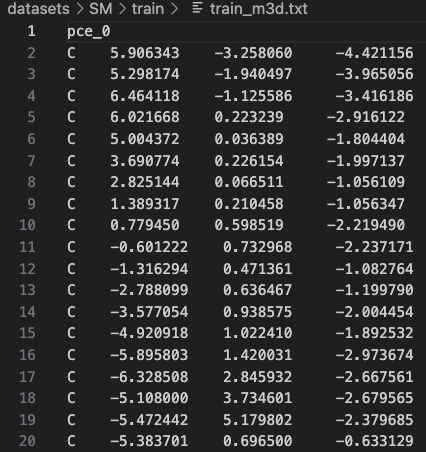
\includegraphics[width=0.4\textwidth]{Datasets/coords.png}
    \caption{Coordonnées 3D d'une molécule}
\end{figure}

Pour chaque molécules, on génére les coordonnées 3D de chaque atomes.
Ensuite on récupère ces coordonnées 3D on effectue un prétraitement  pour les transformer en fichier \texttt{.npy} pour qu'ils puissent enfin être utilisé par le modèle de prédiction.




\newpage

\section{Prérequis}
Pour la suite de ce document, l'ensemble du projet a été réalisé avec un environnement virtuel (conda).

\subsection{Vérification de la présence d'un GPU et installation de CUDA}

Pour profiter de l'accélération matérielle (ce qu'on vous recommande fortement) lors de l'entraînement de modèles, il est important de vérifier si votre ordinateur dispose d'un GPU compatible.

\begin{itemize}
    \item \textbf{Sous Windows :} Ouvrez le gestionnaire de tâches (\texttt{Ctrl+Shift+Esc}) et vérifiez l'onglet ``Performances'' pour voir si un GPU nvidia est détecté.
    \begin{verbatim}
    lspci | grep -i nvidia
    \end{verbatim}
\end{itemize}

\textbf{Installation de CUDA :}

\begin{enumerate}
    \item Rendez-vous sur le site officiel de NVIDIA : \url{https://developer.nvidia.com/cuda-downloads}. Pour l'Installer typeprenez la version local
    \item Sélectionnez votre système d'exploitation et suivez les instructions d'installation.
    \item Après installation, vérifiez la version de CUDA avec la commande :
    \begin{verbatim} 
                        nvcc --version
    \end{verbatim}
\end{enumerate}

\textbf{Remarque :} Assurez-vous que la version de CUDA installée est compatible avec la version de PyTorch que vous souhaitez utiliser (voir la documentation officielle de PyTorch).

\subsection{Installation de Pytorch}
Avant de commencer, munissez vous d'un environnement virtuel et assurez-vous d'avoir installé les dépendances nécessaires. L'ensemble des dépendances se retrouvent dans un fichier \texttt{requirements.txt} et sont facilement installables via \texttt{pip} ou \texttt{conda}.
Activez votre environnement virtuel et vous pourrez commencez à utiliser les commandes \texttt{bash} du guide utilisateur sur votre terminal.
Par ailleurs, une dépendance importante à prendre en compte est la library avec laquelle sont écrit les réseaux de neuronnes profonds : \textbf{\href{https://pytorch.org/get-started/locally/}{Pytorch}}.

\begin{figure}[H]
    \centering
    \href{https://pytorch.org/get-started/locally/}{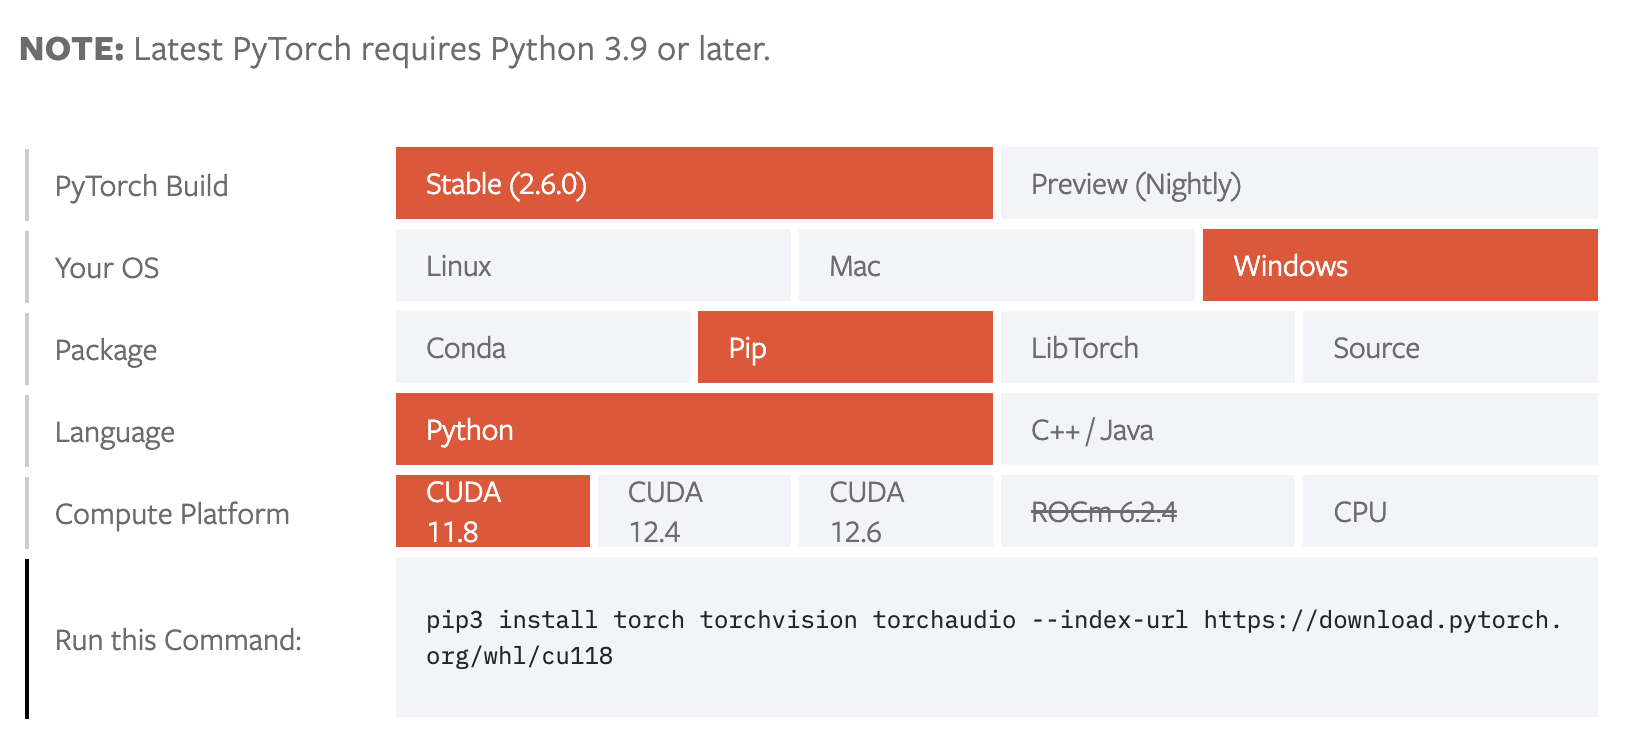
\includegraphics[width=0.6\textwidth]{GuideUtilisateur/pytorch.png}}
    \caption{Page de téléchargement de Pytorch}
\end{figure}

Pour vérifier la disponibilité du GPU avec \texttt{PyTorch}, lancez dans un terminal Python :
\begin{verbatim}
import torch
print(torch.cuda.is_available())
\end{verbatim}
Si la commande retourne \texttt{True}, votre GPU est prêt à être utilisé.

\newpage

\section{Guide utilisateur}
Dans cette section, nous allons vous guider sur la prise main de l'ensemble du projet.
Nous allons vous expliquer comment utiliser le modèle QDF dans les grandes lignes en une série d'étapes pour assurer la cohérence de la pipeline et prédire les propriétés des matériaux donneurs, en particulier le PCE. 
En ce qui concerne l'explication du code des notebooks au format \texttt{.ipynb} ainsi que les commentaires présents dans le code, ont été mis à disposition pour comprendre le fonctionnement de ce derniers.
Aussi,  nous nous accentuerons sur les traitements des deux datasets principaux que sont les PM (polymers molecules) et les SM (small molecules) et comment on parvient à les utiliser dans le modèle.\\
\textbf{NB } : On tient à rappeler que l'ensemble des commandes qui seront présentées par la suite ont été effectuées sur windows.

\subsection{Arbre du projet}

L'Arbre du projet est organisé de manière à faciliter la navigation et l'utilisation des différents composants du projet. Voici un aperçu de la structure de l'arborescence : 

\begin{figure}[H]
    \centering
    \begin{minipage}{0.2\linewidth}
        \begin{forest}
            pic dir tree,
            where level=0{}{% folder icons by default; override using file for file icons
                directory,
            },
            [ProjetDonor
              [data\_preprocess
                [coordinates.py, file]
                [coordinates.sh, file]
                [split\_data.py, file]
                [split\_data.sh, file]
              ]
              [datasets
                [output]
                [data\_test]
                [PM]
                [SM]
              ]
              [model
                [predict]
                [preprocess]
                [train\_model]
              ]
              [VAE]
              [requirements.txt, file]
              [courbe\_apprentissage.py, file]
              [output\_SM.txt ou output\_PM.txt, file]
            ]
          \end{forest}
\end{minipage}
\caption{Arborescence du projet}
\label{fig:arborescence}
\end{figure}

\paragraph{Data\_preprocess :} 
Le dossier \texttt{data\_preprocess} contient les scripts nécessaires pour prétraiter les données. 
En effet, la forme principale des molécules des datasets pour les PM (polymers molecules) et SM (small molecules) sont au format \textbf{SMILES} il va donc falloir les traiter pour les passer sous forme de coordonnées 3D en utilisant \textbf{RdKit}.

\paragraph{Datasets :}
Le dossier \texttt{datasets} contient les dossiers \texttt{PM} et \texttt{SM} eux même qui contiennent chacun les datasets (des PM et SM) encodés sous forme SMILES et les coordonnées 3D associées à ces datasets pour l'entrainement, la validation et le test.
Le dossier \texttt{output} contient les résultats de la prédiction du PCE pour les PM et SM ainsi que les modèles d'entrainement associés.

\paragraph{Model :}
Le dossier \texttt{model} contient les scripts nécessaires pour l'entrainement du modèle QDF, la prédiction du PCE et le preprocess des données réalisés sur les datasets PM.csv et SM.csv.

% \paragraph{VAE :}
% djeci

Avant de commencer à expliquer les principales étapes du projet, il est important de prendre en compte le fait qu'au départ seuls les dossiers \texttt{PM} et \texttt{SM} contenant les fichiers \texttt{PM.csv} et \texttt{SM.csv} sont contenus dans le dossiers datasets. 
Au fur et à mesure qu'on effectue les étapes la strucutre change en rajoutant des dossiers.

\subsection{Séparation du dataset}

La première étape du projet consiste à réaliser une séparation du dataset (PM.csv ou SM.csv) que l'on veut utiliser en trois parties : une partie pour l'entrainement, une partie pour la validation et une partie pour le test.
Pour cela on utilise le script \texttt{split\_data.sh} qui se trouve dans le dossier \texttt{data\_preprocess}.
\\
Le contenu du script \texttt{split\_data.sh} est le suivant :
\begin{figure}[htbp]
    \centering
    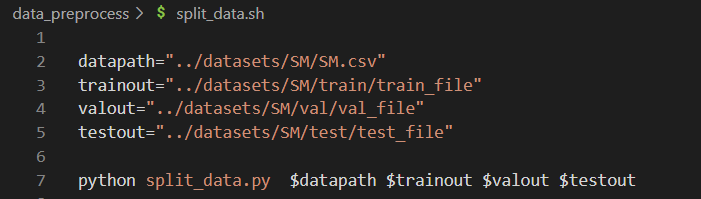
\includegraphics[width=0.6\textwidth]{GuideUtilisateur/split1.png}
    \caption{Contenu du script split\_data.sh}
\end{figure}

Dans cette image on peut voir que l'on utilise le script \texttt{split\_data.py} qui se trouve dans le même dossier. Le premier argument (datapath) est le nom du fichier CSV à traiter (PM.csv ou SM.csv) et les autres arguments sont les noms des des dossiers de sortie.

Pour exécuter le script, il faut ouvrir un terminal \textbf{bash} sur un éditeur comme VS code, accéder au dossier data\_preprocess avec la commande \texttt{cd data\_preprocess} et lancer le scritpt depuis ce terminal avec la commande : \texttt{bash split\_data.sh} sur windows. \\
\textbf{NB} : Si on veut fait un split des données sur le dataset PM il faudra juste remplacer SM par PM.

\subsection{Transformation des SMILES en coordonnées 3D}

La deuxième étape du projet consiste à transformer les SMILES en coordonnées 3D. Pour cela, on utilise le script \texttt{coordinates.sh} qui se trouve dans le dossier \texttt{data\_preprocess}.
Celà permettra d'avoir une base numérique pour l'entrainement des données sur le QDF.  \\
Le script \texttt{coordinates.sh} est le suivant :

\begin{figure}[H]
    \centering
    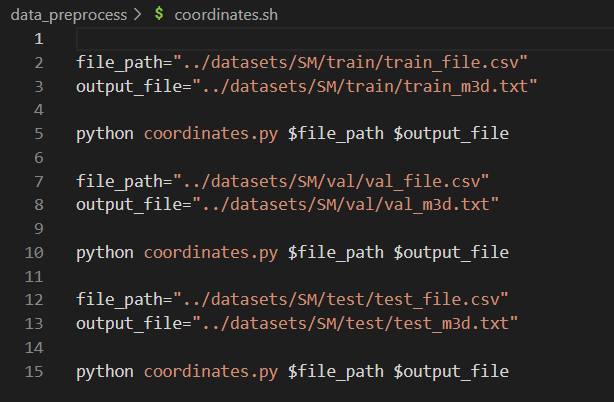
\includegraphics[width=0.6\textwidth]{GuideUtilisateur/coordinates1.png}
    \caption{Contenu du script coordinates.sh}
\end{figure}

Sur l'image on peut voir que chaque variable \texttt{file\_path} correspond au fichier créé lors de la séparation du dataset tandis que les variables \texttt{output\_path} correspondent aux fichiers de sortie qui contiendront les coordonnées 3D des molécules.

\subsection{Préparation des données pour le modèle} 

La troisième étape du projet consiste à préparer les données pour le modèle QDF. Pour cela, on utilise le script \texttt{preprocess.sh} qui se trouve dans le dossier \texttt{model/preprocess}.

\begin{figure}[H]
    \centering
    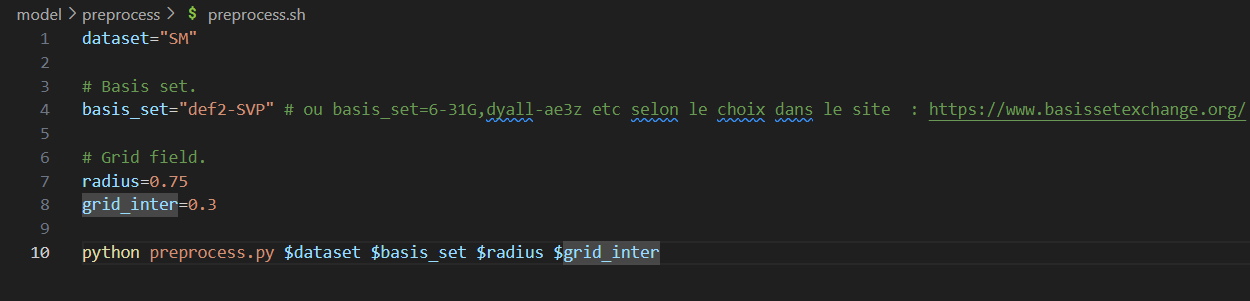
\includegraphics[width=0.8\textwidth]{GuideUtilisateur/preprocess1.png}
    \caption{Contenu du script preprocess.sh}
\end{figure}

La première variable \texttt{dataset} sert à définir le nom du dataset surlequel on souhaite faire du preprocessing. 
La deuxième variable \texttt{basis\_set} sert à définir l'ensemble de fonctions de bases utilisé.
Les variables \texttt{radius} et \texttt{grid\_size} servent à définir le rayon et la taille de la grille utilisée pour le champ électrique associé à chaque atomes.

\subsection{Entrainement du modèle}

La quatrième étape du projet consiste à entrainer le modèle QDF. Pour cela, on utilise le script \texttt{QDF\_SM.sh} ou \texttt{QDF\_PM.sh} qui se trouve dans le dossier \texttt{model/train\_model}.
Un ensemble de plusieurs paramètres sont à définir dans le script \texttt{QDF\_SM.sh} ou \texttt{QDF\_PM.sh} :

\begin{figure}[H]
    \centering
    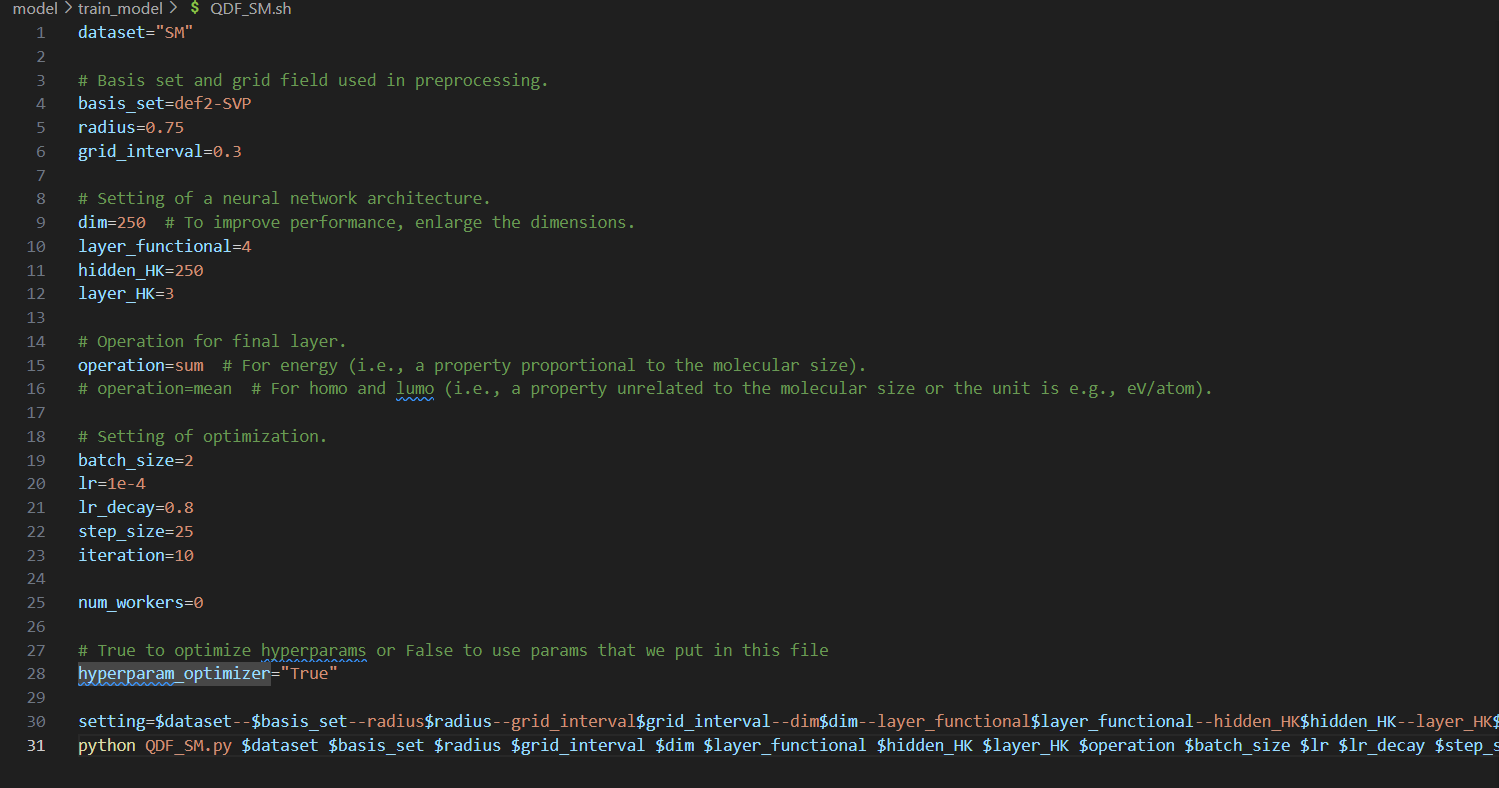
\includegraphics[width=0.8\textwidth]{GuideUtilisateur/train1.png}
    \caption{Variable contenu dans QDF\_SM.sh}
\end{figure}

Une variable importante qui influence la façon dont le modèle va apprendre est \texttt{hyperparam\_optimizer}.
Les hyperparamètres sont enregistrés dans un fichier qui servira de transfert learning pour l'entrainement du modèle QDF pour les PM.

\begin{figure}[H]
    \centering
    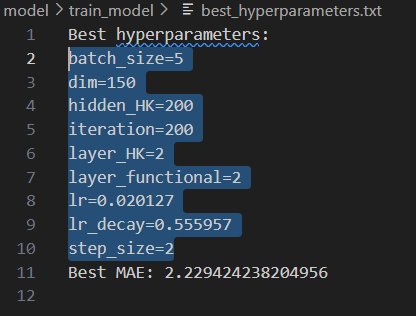
\includegraphics[width=0.3\textwidth]{GuideUtilisateur/hyper1.png}
    \caption{Hyperparamètres optimisés}
\end{figure}

On utilise les hyperparamètres optimisés pour le modèle QDF sur les SM pour entrainer le modèle QDF sur les PM.

\begin{figure}[H]
    \centering
    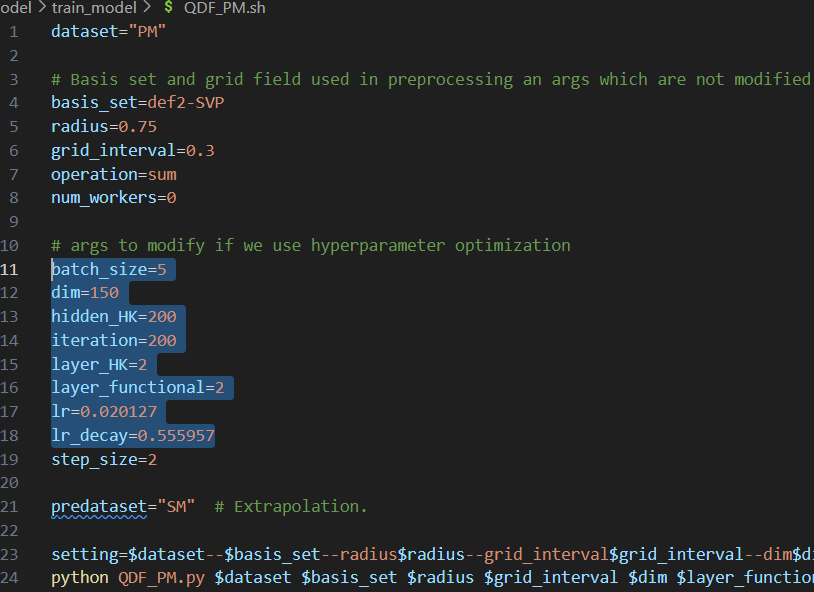
\includegraphics[width=0.6\textwidth]{GuideUtilisateur/pm1.png}
    \caption{Variable contenu dans QDF\_PM.sh}
\end{figure}

Il suffit juste de faire un copier de la partie surligner dans le fichier des hyperparamètres générés lors de l'entrainement du modèle QDF sur les SM et de le coller dans le fichier QDF\_PM.sh.
Les modèles d'entrainement sont sauvegardés dans le dossier \texttt{datasets/output}.

\subsection{Prédiction du PCE}

La dernière étape du projet pour le modèle de prédiction consiste à prédire le PCE des PM et SM grâce au modèle qu'on a pu entrainer. Pour cela, on utilise le script \texttt{predict.sh} qui se trouve dans le dossier \texttt{model/predict}.
Avant cela, il y a un prétraitement de données à faire , si les données reçues sont sous forme de SMILES, avec le script \texttt{preprocess\_predict.sh} se trouvant dans le même répertoire que \texttt{model/predict}. 

\subsection{Courbe d'apprentissage}

La courbe d'apprentissage est un outil essentiel pour évaluer la performance d'un modèle au fil du temps. 
Pour pouvoir la visualiser, il faut exécuter script python \texttt{courbe\_apprentissage.py} qui se trouve à la racine. 
Avant de le faire il faudrait s'assurer que le fichier \texttt{output\_SM.txt ou output\_PM.txt} contiennent des données si ce n'est pas le cas il faut aller dans dossier \texttt{datasets/output} et faire un copier-coller du fichier \texttt{SM--def2-SVP--radius0.75...} dans output\_SM.txt ou output\_PM.txt.

\begin{figure}[H]
  \centering
  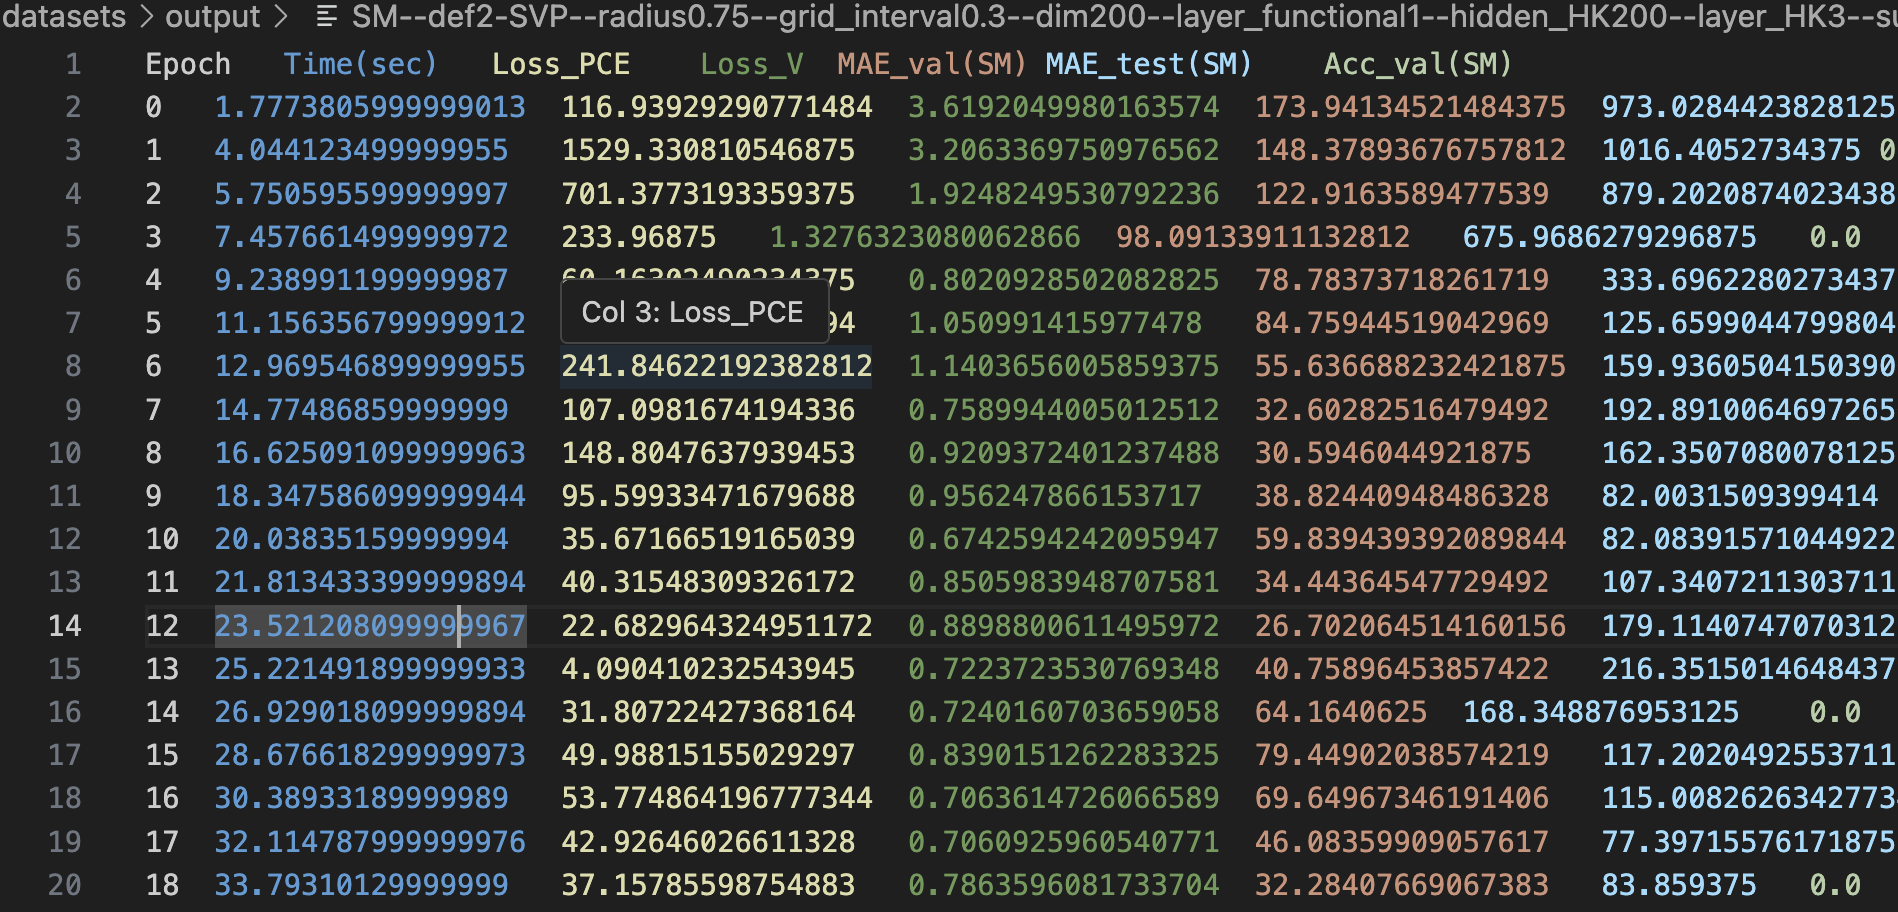
\includegraphics[width=0.6\textwidth]{GuideUtilisateur/train2.png}
  \caption{Contenu des données d'entrainement de datasets/ouput à copier-coller}
\end{figure}

On peut voir sur le graphe que les métrics utilisés pour ce modèle sont la perte et l'accuracy.

\subsection{Demo pour le modèle de prédiction}

En ce qui concerne la démo pour le modèle de prédiction, l'utilisateur pourra exécuter les fichiers \texttt{.ipynb} qui se trouvent dans les dossiers \texttt{data\_preprocess} et \texttt{model/preprocess} dans l'ordre des étapes décrites précédemment.
Une fois traitement des données réalisés une autre notebook présent dans le dossier \texttt{model/train\_model} sert uniquement à expliquer certaines composantes du projet. 
Pour avoir une démonstration de l'entrainement, faire du transfert learning et prédire il faudrait alors utiliser les scripts \texttt{QDF\_SM.sh} et \texttt{QDF\_PM.sh} qui se trouvent dans le dossier \texttt{model/train\_model} ainsi que ceux dans le dossier \texttt{predict}.

\subsection{VAE}
Le pipeline d'entraînement est structuré en plusieurs modules opérationnels :

\begin{itemize}
    \item \textbf{Chargement et nettoyage} : lecture des fichiers, suppression des erreurs et normalisation.
    \item \textbf{Encodage vectoriel} : transformation des SMILES en séquences compatibles avec le réseau neuronal.
    \item \textbf{Modélisation} : apprentissage d'une représentation latente des molécules à l'aide d'un modèle génératif.
    \item \textbf{Prédiction} : estimation de la Power Conversion Efficiency (PCE) en sortie du modèle.
    \item \textbf{Analyse et visualisation} : évaluation des performances, affichage graphique, génération de nouvelles structures.
\end{itemize}

Pour pourvoir exécuter le modèle, il faur se rendre dans le dossier \texttt{VAE} et exécuter le script \texttt{vae\_essaie.py} qui se trouve dans ce dernier depuis un terminal bash avec \texttt{python vae\_essaie.py} en activant l'environnement virtuel avant.
Un notebook est présent pour expliquer les fonctions du modèle en plus des commentaires.

% En lisant cette section, le lecteur devrait être en mesure de comprendre comment utiliser le modèle QDF pour prédire les propriétés des matériaux donneurs, en particulier le PCE. 
% Maintenant nous allons vous donnez une vue d'ensemble sur les libraries utilisé et le code pour ce projet.


\subsection{Conseils d'utilisation}

\subsubsection{GPU}
Lors de l'entrainement du modèle de prédiction, il est crucial d'utiliser un GPU suffisamment puissant et de disposer d'une quantité de mémoire RAM adaptée, que ce soit sur un PC personnel ou sur un serveur distant. En effet, l'entraînement de modèles de deep learning, en particulier sur des jeux de données volumineux ou des architectures complexes, nécessite des ressources matérielles importantes pour garantir des temps de calcul raisonnables et permettre l'utilisation de batchs de grande taille.
Pour l'entrainement de notre modèle de prédiction on a utilisé un server en ligne (OVHCloud) avec une \textbf{NVIDIA L40 S} avec 45 Go de mémoire GPU. 

\subsubsection{Basis set}
Le choix de la base de fonction est important pour la prédiction du PCE. 
Pour ce projet on a utilisé la base de fonction \textbf{def2-SVP} mais il est possible de le changer en fonction de la préférence. 
On l'a utilisé dans ce projet, car il couvrait un grand nombre d'élément chimique et est plus précis que le \textbf{6-31G}.



\newpage

\section{Axes d'amélioraitons}

\subsection{Suggestion modèle de prédiction}

\subsubsection{GPU}

Comme il a été mentionné précédemment, on utilise une \textbf{Nvidia L40 S}.
Même avec cette configuration, on est limité en ce qui concerne la \textbf{batch\_size} de notre modèle. 
La taille du lot (batch size) est un hyperparamètre qui détermine le nombre d'échantillons à traiter avant de mettre à jour les poids du modèle.
Pour l'augmenter, il faudrait utiliser plusieurs GPU et faire probablement de l'entrainement distribué pour permette de traiter plusieurs lots et potentiellement améliorer le modèle.

\textbf{NB :} Si il le GPU n'est pas assez puissant lors de l'exéction du modèle, il serai possible que des erreurs liés à la mémoire apparaissent. Souvent des erreurs de type \texttt{CUDA out of memory} apparaissent.

\subsubsection{Hyperparamètres}
Pour ce projet, on a utilisé un algorithme d'optimisation des hyperparamètres (ex : batch\_size) via la librairie \texttt{hyperopt}.
Cependant, on a été limité en termes de temps ce qui a valu une dimunution de l'espace de recherche de ces hyperparamètres.  
À l'avenir il serait utile d'agrandir l'espace de recherche des hyperparamètres avec des valeurs plus grandes dans l'espace de recherche pour étendre la recherche des meilleures hyperparamètres.

\begin{figure}[H]
    \centering
    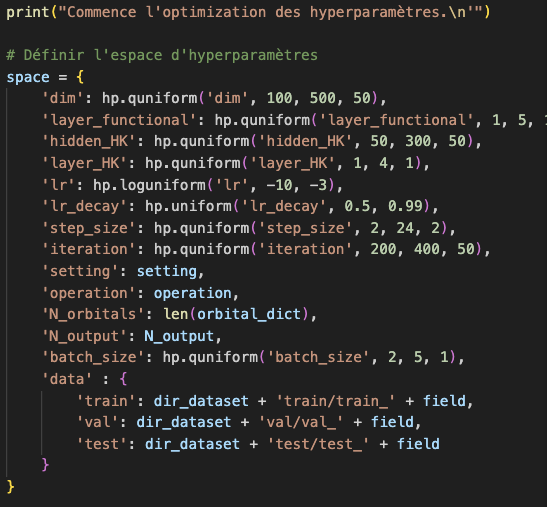
\includegraphics[width=0.6\textwidth]{Overview/hyper.png}
    \caption{Espace de recherche des Hyperparamètres}
\end{figure}

\subsubsection{Fonction de pertes du modèle}
La fonction de perte est un élément clé dans l'entraînement d'un modèle d'apprentissage automatique.
Elle mesure la différence entre les prédictions du modèle et les valeurs réelles.
Dans le cas de la prédiction de PCE, la fonction de perte utilisée est la \textbf{MAE} (Mean Absolute Error).
Le MAE est une mesure linéaire de la différence entre les valeurs prédites et les valeurs réelles.
Pour espérer mieux extrapoler les données, il serait intéressant d'utiliser une fonction de perte non linéaire comme la \textbf{Huber Loss ou RMSE} qui est moins sensible aux valeurs aberrantes que la MAE.

\subsection{Modèle de génération}

\subsubsection{Traduction SMILES en SELFIES}

L'une des principales difficultés rencontrées concerne la conversion des représentations SMILES en SELFIES (Self-Referencing Embedded Strings). Bien que SELFIES soit plus robuste pour la génération de structures valides, sa conversion depuis des SMILES complexes n’est pas toujours triviale. Certains encodages échouent ou génèrent des représentations ambiguës, nécessitant une étape supplémentaire de validation et de correction. Cela introduit une complexité additionnelle dans le pipeline de traitement et peut réduire la qualité des entrées pour le modèle génératif.

\subsubsection{Génération de molécules via NO-Operation (NOP)}

Lors de la génération de nouvelles structures moléculaires, nous avons observé que certains modèles avaient tendance à produire un grand nombre de caractères de type NO-Operation (NOP), c’est-à-dire des éléments neutres ou répétitifs sans signification chimique. Cela peut résulter d’un mauvais apprentissage des règles syntaxiques moléculaires ou d’un sur-apprentissage sur les motifs fréquents. La présence excessive de NOP réduit la diversité et la qualité des molécules générées, ce qui compromet leur validité et leur pertinence.


\newpage

\section{Appendices}


\subsection{References}


\sloppy % Permet de réduire les avertissements liés à la mise en page

\begin{thebibliography}{9}

\bibitem{Sun}
Jinyu Sun, Dongxu Li, Yue Wang, Ting Xie, Yingping Zou, Hongmei Lu and Zhimin Zhang, \textit{J. Mater. Chem. A}, 2024,  DOI: 10.1039/D4TA03944K


\bibitem{Masashi}
Tsubaki, Masashi and Mizoguchi, Teruyasu, \textit{Quantum Deep Field: Data-Driven Wave Function, Electron Density Generation, and Atomization Energy Prediction and Extrapolation with Machine Learning}, Phys. Rev. Lett. \textbf{125}(20):206401, 2020, doi: 0.1103/PhysRevLett.125.206401 % \href{https://doi.org/10.1103/PhysRevLett.125.206401}{1}.

\end{thebibliography}



\subsection{Définitions additionnelles ou figures complémentaires}

\textbf{InChI (Identifiant International des Composés Chimiques)}

\begin{description}
  \item[Définition :] Une représentation textuelle normalisée d'une molécule chimique, offrant une structure plus rigoureuse que SMILES.

  \item[Exemple :]
  Benzène : \texttt{InChI=1S/C6H6/c1-2-4-6-5-3-1/h1-6H}
\end{description} 

\vspace{0.25cm}

\noindent \textbf{Orbitales de type gaussien (GTOs)}
\begin{description}
  \item[Définition :] Une Orbitale de Type Gaussien (GTO) est une fonction mathématique utilisée comme fonction de base en chimie quantique pour approximer les orbitales atomiques. Au lieu d'utiliser une décroissance exponentielle pure, les GTOs emploient une fonction gaussienne, ce qui simplifie le calcul des intégrales dans les calculs de structure électronique moléculaire.

  % Formule : \[
  %   \chi(x) = N x^{l} e^{-\alpha x^{2}}
  %   \]
  Formule : \[
    \phi(r) = R_{l}(r) Y_{lm}(\theta, \phi)
  \]

  \item[\(\phi(x)\) :] La fonction orbitale unidimensionnelle, où \(x\) est la coordonnée spatiale.
  \item[\( R_{l}(r) = N r^{l} e^{-\alpha r^{2}} \) :] La partie radiale du GTO, où \(r\) est la distance au noyau.
  \item[\(N\) :] La constante de normalisation.
  \item[\(l\) :] Un entier positif ou nul déterminant le type (par exemple, \(l=0\) pour s, \(l=1\) pour p).
  \item[\(\alpha\) :] Un paramètre positif contrôlant l'étalement (largeur) de la gaussienne.
  \item[\(e^{-\alpha r^{2}}\) :] La partie gaussienne, assurant une décroissance rapide lorsque \(|r|\) augmente.
  \item[\(Y_{lm}(\theta, \phi)\) :] Les harmoniques sphériques, qui dépendent des angles \(\theta\) et \(\phi\) et décrivent la partie angulaire de l'orbitale.
\end{description}

\vspace{0.25cm}

\noindent \textbf{Autoencodeur variationnel : VAE}
\begin{description}
  \item[Définition :] Un autoencodeur variationnel est un modèle génératif profond utilisé en apprentissage automatique. Il apprend une représentation latente probabiliste des données d'entrée à l'aide de deux réseaux de neurones :
  \item Un \textbf{encodeur} qui projette les données d'entrée vers une distribution latente.
  \item Un \textbf{décodeur} qui échantillonne à partir de cette distribution latente pour générer de nouvelles données similaires à l'ensemble d'entraînement.

  \item Les VAE sont particulièrement utiles pour générer de nouvelles structures (molécules, etc.) et explorer l'espace afin de découvrir des motifs intéressants.
\end{description}

\vspace{0.25cm}

\noindent \textbf{Réseau de neurones profond : DNN}
\begin{description}
  \item[Définition :] Un réseau de neurones profond (DNN) est un réseau de neurones artificiel composé de plusieurs couches de neurones entre l'entrée et la sortie. Contrairement à un réseau simple avec une ou deux couches cachées, un DNN contient un grand nombre de couches cachées qui lui permettent de modéliser des relations très complexes et de détecter des motifs subtils dans les données. Cela le rend très efficace pour de nombreuses tâches, telles que la reconnaissance d'images, la traduction automatique et la prédiction de comportements.
\end{description}

\vspace{0.25cm}

\noindent \textbf{Quantum Deep Field : QDF}
\begin{description}
  \item[Définition :] Le Quantum Deep Field (QDF) est une méthode qui combine la chimie quantique avec des réseaux de neurones profonds pour prédire les propriétés de molécules ou de matériaux. Elle utilise des informations issues de calculs quantiques (telles que les distributions électroniques) et les intègre dans un modèle d'apprentissage profond, permettant des prédictions plus précises et fiables que les approches traditionnelles.
\end{description}

\noindent \textbf{PCE : Rendement de conversion de puissance}
\begin{description}
  \item[Définition :] Le rendement de conversion de puissance (PCE, pour Power Conversion Efficiency) est une mesure de l'efficacité avec laquelle un dispositif (par exemple, une cellule solaire) convertit l'énergie incidente (comme la lumière) en énergie utilisable (comme l'électricité).
\end{description}

\noindent \textbf{Fonctionnelles}
\begin{description}
  \item[Définition :] En chimie quantique, une fonctionnelle est une fonction qui prend une fonction (par exemple, la densité électronique) comme argument et retourne une valeur scalaire. Les fonctionnelles sont essentielles dans la théorie de la fonctionnelle de la densité (DFT) pour approximer l'énergie totale d'un système.
\end{description}

\noindent \textbf{Base de fonctions (Basis-set)}
\begin{description}
  \item[Définition :] Un ensemble de base (basis-set) est un ensemble de fonctions mathématiques utilisées pour décrire les orbitales électroniques dans les calculs de chimie quantique. Le choix de l'ensemble de base influence la précision et le coût des calculs.
\end{description}



\end{document}
